\documentclass[reqno,a4paper,12pt]{amsart}

\usepackage{amsmath,amssymb,amsthm,geometry,xcolor,soul,graphicx}
%\usepackage{array}
\usepackage{float} % 在tcolorbox中添加table (由于tcolorbox已经是一个box,因此不能直接加table)
\usepackage{titlesec}
%\usepackage{enumitem}
\usepackage{enumerate}
\usepackage{lipsum}
\usepackage{listings}
\allowdisplaybreaks[4] %align公式跨页
\RequirePackage[most]{tcolorbox}
%\usepackage{braket}
%\usepackage{esint} %$\varoiint$ (带圈的二重积分)
%\usepackage[colorlinks,linkcolor=red]{hyperref} %\url{}超链接
\usepackage[scheme=plain,linespread=1,punct=CCT]{ctex}% Chinese support, single line space, narrow-version SBC case punctuations
\setCJKfamilyfont{zhsong}[AutoFakeBold={2.17}]{SimSong-Regular}
\renewcommand{\songti}{\CJKfamily{zhsong}}
%\usepackage{xeCJK}
%\setCJKmainfont{Kai}
\geometry{left=0.7in, right=0.7in, top=1in, bottom=1in}

\renewcommand{\baselinestretch}{1.3}

\title{固体物理第八次作业}
\author{董建宇 ~~ 2019511017}

\begin{document}

\maketitle
\titleformat{\section}[hang]{\small}{\thesection}{0.8em}{}{}
\titleformat{\subsection}[hang]{\small}{\thesubsection}{0.8em}{}{}

\begin{enumerate}[1.]
\item \textbf{(14.2) $\ddagger$ X-ray scattering II} \\
$BaTiO_3$ has a primitive cubic lattice and a basis with atoms having fractional coordinates 
\[
\begin{array}{llll}
	Ba & [0,0,0] &  &  \\
	Ti & [0.5,0.5,0.5] &  &  \\
	O & [0.5,0.5,0], & [0.5,0,0.5], & [0,0.5,0.5]
\end{array}
\]
$\triangleright$ Sketch the unit cell. \\
$\triangleright$ Show that the X-ray structure factor for the $(00l)$ Bragg reflections is given by 
\[
	S(hkl) = f_{Ba} + (-1)^l f_{Ti} + \left[ 1+2(-1)^l \right]f_O
\]
where $f_{Ba}$ is the atomic form factor for Ba, etc. \\
$\triangleright$ Calculate the ratio $I_{002}/I_{001}$, where $I_{(hkl)}$ is the intensity of the X-ray diffraction from the $(hkl)$ planes. You may assume that the atomic form factor is proportional to atomic number (Z), and neglect its dependence on the scattering vector. $(Z_{Ba} = 56, Z_{Ti} = 22, Z_O = 8.)$

\begin{tcolorbox}[breakable, colback = black!5!white, colframe = black]
$\triangleright$ 利用VESTA绘制元胞如下图: \\
\begin{centering}
	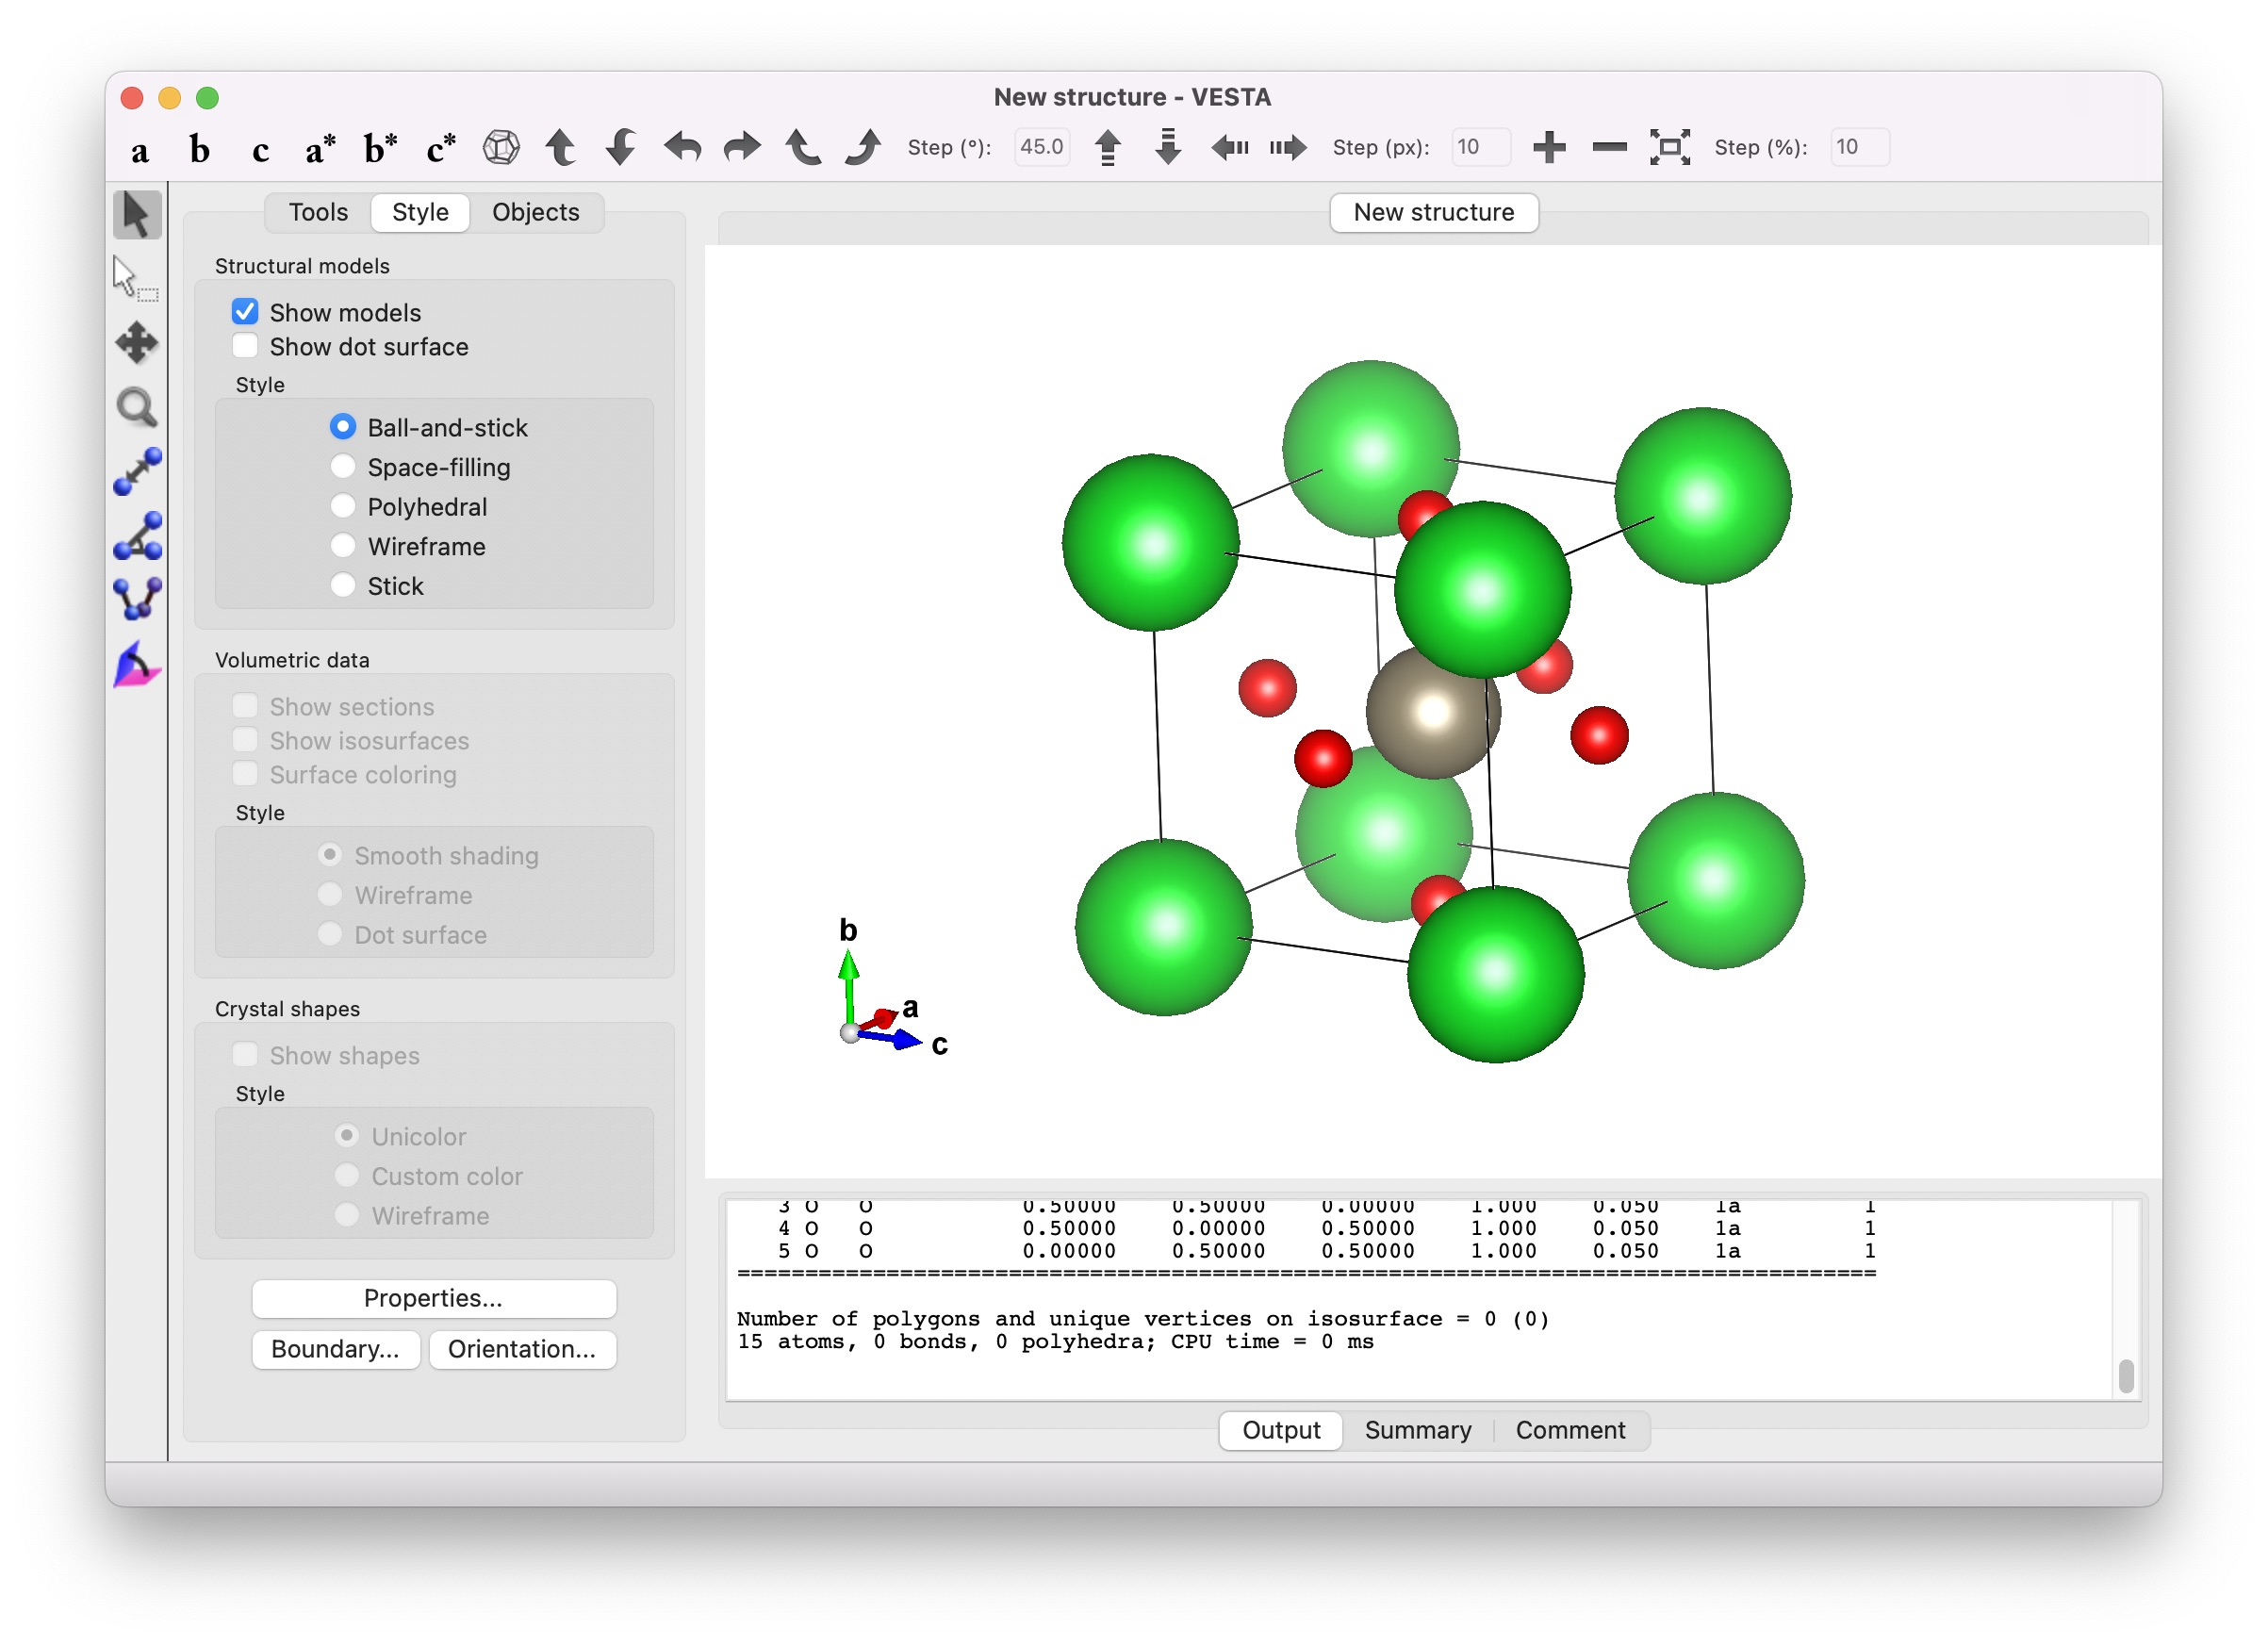
\includegraphics[scale = 0.15]{14.2.jpeg}
\end{centering}\\
其中,位于顶点处的绿色原子为$Ba$,位于体心的棕色原子为$Ti$,位于面心的红色原子为$O$。 \\
$\triangleright$ 对于$(00l)$Bragg反射的结构因子为:
\[
	S_{(00l)} = f_{Ba} + e^{i\vec{G}\cdot\vec{r}_{Ti}} f_{Ti} + \sum_{n=1}^3 e^{i\vec{G} \cdot \vec{r}_{O_n}} f_O.
\]
上式中,$\vec{G}\cdot\vec{r}$由下面给出: 
\begin{align*}
	\vec{G}\cdot\vec{r}_{Ti} =& l\vec{b}_3 \cdot \frac{\vec{a_1} + \vec{a}_2 + \vec{a}_3}{2} = l \pi, \\
	\vec{G}\cdot\vec{r}_{O_1} =& l\vec{b}_3 \cdot \frac{\vec{a_1} + \vec{a}_2}{2} = 0, \\
	\vec{G}\cdot\vec{r}_{O_2} =& l\vec{b}_3 \cdot \frac{\vec{a_1} + \vec{a}_3}{2} = l \pi, \\
	\vec{G}\cdot\vec{r}_{O_3} =& l\vec{b}_3 \cdot \frac{\vec{a_2} + \vec{a}_3}{2} = l \pi.
\end{align*}
则结构因子为:
\[
	S_{(00l)} = f_{Ba} + e^{il\pi} f_{Ti} + (1+2e^{il\pi})f_O = f_{Ba} + (-1)^l f_{Ti} + \left[ 1+2(-1)^l \right]f_O.
\]
$\triangleright$ 假设原子的形状因子正比于原子序数,则可以计算:
\[
	\frac{I_{002}}{I_{(001)}} = \frac{\vert S_{(002)} \vert^2}{\vert S_{(001)} \vert^2} = \frac{\vert f_{Ba} + f_{Ti} +3f_O \vert^2}{\vert f_{Ba} - f_{Ti} - f_{O} \vert^2} = \frac{2601}{169} \approx 15.4
\]
\end{tcolorbox}

\item \textbf{(14.3) $\ddagger$ X-ray scattering and Systematic Absences} \\
(a) Explain what is meant by "Lattice Constant" for a cubic crystal structure. \\
(b) Explain why X-ray diffraction may be observed in first order from the (110) planes of a crystal with a body-centered cubic lattice, but not from the (110) planes of a crystal with a face-centered cubic lattice. \\
$\triangleright$ Derive the general selection rules for which planes are observed in bcc and fcc lattices. \\
(c) Show that these selection rules hold independent of what atoms are in the primitive unit cell, so long as the lattice is bcc or fcc respectively. \\
(d) A collimated beam of monochromatic X-rays of wavelength $0.162$ nm is incident upon a powdered sample of the cubic metal palladium. Peaks in the scattered X-ray pattern are observed at angles of $42.3^{\circ}$, $49.2^{\circ}$, $72.2^{\circ}$, $87.4^{\circ}$, and $92.3^{\circ}$ from the direction of incident beam. \\
$\triangleright$ Identify the lattice type. \\
$\triangleright$ Calculate the lattice constant and the nearest neighbor distance. \\
$\triangleright$ If you assume there is only a single atom in the basis does this distance agree with the known data that the density of palladium is $12023 kg~m^{-3}$? (Atomic mass of palladium = 106.4) \\
(e) How could you improve the precision with which the lattice constant is determined. (For one suggestion, see Exercise 14.10.)
\vspace{2ex}
\begin{tcolorbox}[breakable, colback = black!5!white, colframe = black]
\begin{enumerate}[(a)]
\item 对于立方晶格,晶格常数为最近邻两个周围环境相同的原子间距离。

\item 对于体心立方结构,(110)平面包含了所有的原子;而对于面心立方晶体,(110)平面只包含了一半原子,而恰好未被包含的原子的散射波与被包含的原子的散射波可以一一对应干涉相消,所以对于面心立方晶体看不到X射线在(110)截面的散射。 \\
$\triangleright$ 对于面心立方晶体,结构因子可以写为:
\[
	S_{(hkl)} = f \left( 1+e^{i\pi(h+k)} + e^{i\pi(h+l)} + e^{i\pi(k+l)} \right) = f(1+(-1)^{h+k} + (-1)^{h+l} + (-1)^{k+l}).
\]
令$S_{(hkl)} \neq 0$,有:$h,k,l$全部为奇数或者全部为偶数。 \\
对于体心立方晶体,结构因子可以写为:
\[
	S_{(hkl)} =  f \left( 1+e^{i\pi(h+k+l)} \right) = f(1+(-1)^{h+k+l}).
\]
令$S_{(hkl)} \neq 0$,有:$h+k+l$为偶数。 \\

\item 假设原初晶包中存在$n$个原子,位置做标记为$\vec{r}_i$,其中$i=1,2,\cdots,n$。记$A_i$表示第$i$个原子,形状因子记为$f_i$。 \\
对于面心立方晶体,结构因子为:
\[
	S_{(hkl)} = (1 + (-1)^{h+k} + (-1)^{h+l} + (-1)^{k+l})\sum_{i=1}^n f_i e^{i\vec{G}\cdot\vec{r}_i}
\]
对于体心立方晶体,结构因子为:
\[
	S_{(hkl)} = (1 + (-1)^{h+k+l})\sum_{i=1}^n f_i e^{i\vec{G}\cdot\vec{r}_i}
\]
即选择定则与原初晶包中原子互相独立,对于面心立方晶体与体心立方晶体上述选择定则仍然成立。 

\item 利用Bragg公式,将提供所给数据列表如下:
\begin{table}[H]
	\centering
	\begin{tabular}{|c|c|c|}
	\hline
	2$\theta$ & $\frac{\lambda}{2\sin\theta}$ & The smallest $n$ to make $\left(\frac{n\lambda}{2\sin\theta}\right)^2$ be equal \\ \hline
	$42.3^{\circ}$ & $0.224nm$ & 3 \\ \hline
	$49.2^{\circ}$ & $0.195nm$ & 4 \\ \hline
	$72.2^{\circ}$ & $0.137nm$ & 8 \\ \hline
	$87.4^{\circ}$ & $0.117nm$ & 11 \\ \hline
	$92.3^{\circ}$ & $0.112nm$ & 12 \\ \hline
	\end{tabular}
\end{table}
则我们可以写出5个倒空间中点的坐标:$(1,1,1);(2,0,0);(2,2,0);(3,1,1);(2,2,2)$,注意到所有坐标全为奇数或全为偶数,则该晶体为面心立方晶体。 \\
$\triangleright$ 可以计算晶格常数为:
\[
	a = \frac{\lambda}{2\sin(21.15^\circ)} \sqrt{1^2+1^2+1^2} = 0.389nm.
\]
最近邻原子间距为:
\[
	s = \frac{a}{\sqrt{2}} = 0.275nm.
\]
$\triangleright$ 如果假设每个原胞中只含有一个原子,可以计算密度为:
\[
	\rho = \frac{4m_0}{a^3} = \frac{4M}{a^3N_A} \approx \frac{4\times106.4\times10^{27}}{N_A\times.89^3}kg\cdot m^{-3} \approx 12006 kg\cdot m^{-3}.
\]
与已知的钯的密度相似。 \\

\item $\bullet$ 根据Bragg公式,可以计算得:
\[
	\frac{1}{d}\frac{d}{d\theta}d = -\frac{1}{\tan\theta}.
\]
当$\theta \to \pi/2$时,$\frac{1}{d}\frac{d}{d\theta}d \to 0$。即在实验中尽可能选取更大的$\theta$,进而计算晶格常数。 \\
$\bullet$ 更精确地确定使用的X射线波长。 \\
$\bullet$ 采取必要的散热措施,避免样品晶格常数受温度影响较大。
\end{enumerate}
\end{tcolorbox}

\item \textbf{(14.5) And More X-ray Scattering}\\
A sample of aluminum powder is put in an Debye-Scherrer X-ray diffraction device. The incident X-ray radiation is from Cu-Ka X-ray transition (this just means that the wavelength is $\lambda = 0.154nm$). The following scattering angles were observed: \\$19.48^{\circ};~ 22.64^{\circ};~ 33.00^{\circ};~ 39.68^{\circ};~ 41.83^{\circ};~ 50.35^{\circ};~ 57.05^{\circ};~ 59.42^{\circ};$ \\
Given also that the atomic weight of Al is 27, and the density is $2.7g/cm{3}$, use this information to calculate Avagadro's number. How far off are you? What causes the error?

\begin{tcolorbox}[breakable, colback = black!5!white, colframe = black]
利用Bragg公式,将提供的数据列表如下:
\begin{table}[H]
	\centering
	\begin{tabular}{|c|c|c|}
	\hline
	$\theta$ & $\frac{\lambda}{2\sin\theta}$ & The smallest $n$ to make $\left(\frac{n\lambda}{2\sin\theta}\right)^2$ be equal \\ \hline
	$19.48^{\circ}$ & $0.2309nm$ & 3 \\ \hline
	$22.64^{\circ}$ & $0.2000nm$ & 4 \\ \hline
	$33.00^{\circ}$ & $0.1414nm$ & 8 \\ \hline
	$39.68^{\circ}$ & $0.1206nm$ & 11 \\ \hline
	$41.83^{\circ}$ & $0.1155nm$ & 12 \\ \hline
	$50.35^{\circ}$ & $0.1000nm$ & 16 \\ \hline
	$57.05^{\circ}$ & $0.0918nm$ & 19 \\ \hline
	$59.42^{\circ}$ & $0.0894nm$ & 20 \\ \hline
	\end{tabular}
\end{table}
则我们可以写出倒空间中点的坐标为:$(1,1,1)$; $(2,0,0)$; $(2,2,0)$; $(3,1,1)$; $(2,2,2)$; $(4,0,0)$; $(3,3,1)$; $(4,2,0)$。注意到所有坐标全为奇数或全为偶数,则该晶体为面心立方晶体。则在常规晶包中存在4个原子,晶格常数为:
\[
	a = \frac{\lambda}{2\sin(19.48^\circ)} \sqrt{3} = 0.400 nm.
\]
利用密度与相对原子质量可以估算Avagadro常数为:
\[
	\hat{N}_A = \frac{4M}{\rho a^3} \approx 6.25\times 10^{23} mol^{-1}.
\]
相对误差为:
\[
	\beta = \frac{\hat{N}_A - N_A}{N_A} \times 100\% \approx 3.78\%.
\]
误差可能来源: \\
$\bullet$ 铝的相对原子质量有效位数较小,从而导致$M$比真实值较大。 \\
$\bullet$ 可能测量密度时的温度与进行X射线衍射时温度不同,导致对Avagadro常数估计出现误差。
\end{tcolorbox}

\item \textbf{(14.9) Form Factors} \\
(a) Assume that the scattering potential can be written as the sum over the contributions of the scattering from each of the atoms in the system. Write the positions of the atoms in terms of a lattice plus a basis so that 
\[
	V(\mathbf{x}) = \sum_{\mathbf{R}, \alpha} V_\alpha(\mathbf{x} - \mathbf{R} - \mathbf{y}_\alpha)
\]
where \textbf{R} are lattice points, $\alpha$ indexes the particles in the basis and $\mathbf{y}_\alpha$ is the position of atom $\alpha$ in the basis. Now use the definition of the structure factor Eq. 14.5 and hence derive expression 14.9 for the form factor. (Hint: Use the fact that an integral over all space can be decomposed into a sum over integrals of individual unit cells.) \\ 
(b) Given the equation for the form factor you just derived (Eq. 14.9), assume the scattering potential from an atom is constant inside a radius $a$ and is zero outside that radius. Derive Eq. 14.10. \\
(c)* Use your knowledge of the wave-function of an electron in a hydrogen atom to calculate the X-ray form factor of hydrogen.
\begin{tcolorbox}[breakable, colback = black!5!white, colframe = black]
\begin{enumerate}[(a)]
\item 结构因子可以写为:
\begin{align*}
	S(\mathbf{G}) =& \int_{unit~cell} \mathbf{dx} e^{i\mathbf{G} \cdot \mathbf{x}} V(\mathbf{x}) \\
	=& \sum_{\mathbf{R},\alpha} \int_{unit~cell} \mathbf{dx} e^{i\mathbf{G} \cdot \mathbf{x}} V_\alpha(\mathbf{x}-\mathbf{R}-\mathbf{y}_\alpha) \\
	=& \sum_{\mathbf{R},\alpha} \int_{unit~cell} \mathbf{dx} e^{i\mathbf{G} \cdot \mathbf{y}_\alpha} e^{i\mathbf{G} \cdot (\mathbf{x}-\mathbf{R}-\mathbf{y}_\alpha)} V_\alpha(\mathbf{x}-\mathbf{R}-\mathbf{y}_\alpha) \\
	=& \sum_{\alpha} e^{i\mathbf{G}\cdot\mathbf{y}_\alpha} \int_{all~space} \mathbf{d(x-R-}\mathbf{y}_\alpha\mathbf{)} e^{i\mathbf{G} \cdot (\mathbf{x}-\mathbf{R}-\mathbf{y}_\alpha)} V_\alpha(\mathbf{x}-\mathbf{R}-\mathbf{y}_\alpha) \\
	=& \sum_{\alpha} e^{i\mathbf{G}\cdot\mathbf{y}_\alpha} \int_{all~space} \mathbf{dr} e^{i\mathbf{G}\cdot\mathbf{r}} V_\alpha(\mathbf{r}) \\
	=& \sum_\alpha e^{-\mathbf{G}\cdot\mathbf{y}_\alpha} f_\alpha(\mathbf{G})
\end{align*}
其中利用了$e^{i\mathbf{G}\cdot\mathbf{R}} = 1$,以及令$f_\alpha(\mathbf{G}) = \int_{all~space} \mathbf{dr} e^{i\mathbf{G}\cdot\mathbf{r}} V_\alpha(\mathbf{r})$。
\item 由题意可令:
\[
	V(r) = \left\{ \begin{array}{ll}
		V_0, & r\leq a; \\
		0, & r>a.
	\end{array} \right.
\]
则形状因子为:
\begin{align*}
	f(\mathbf{G}) =& \int_0^a \int_0^\pi \int_0^{2\pi} e^{iGr\cos\theta} V_0 r^2\sin\theta \,d\phi\,d\theta,\,dr \\
	=& 2\pi V_0 \int_0^a \frac{2}{G}r\sin(Gr) \\
	=& \frac{4\pi V_0}{G} \left( \frac{\sin(Ga)}{G^2} - \frac{a\cos(Ga)}{G} \right) \\
	=& 4\pi V_0 a^3\frac{\sin(Ga) - Ga\cos(Ga)}{(Ga)^3} \\
	=& 4\pi V_0 a^3 \frac{\sin x - x\cos x}{x^3}
\end{align*}
其中$x = Ga$。因为原子核周围势函数正比于核电荷数$Z_j$,则有:
\[
	f(\mathbf{G}) \propto 3Z_j \frac{\sin x - x\cos x}{x^3}.
\]
\item 归一化后的氢原子基态波函数为:
\[
	\psi(r) = Y_{00}R_{10} = \frac{1}{\sqrt{4\pi}}\frac{2}{a_0^{3/2}} e^{-r/a_0}.
\]
势能函数正比于波函数模平方,设比例系数为k,则有:
\[
	V(r) = k\vert \psi(r) \vert^2 = \frac{k}{\pi a_0^3} e^{-2r/a_0}.
\]
则形状因子为:
\begin{align*}
	f(\vec{G}) =& \int \,d\vec{r} e^{i\vec{G} \cdot \vec{r}} V(r) \\
	=& \frac{k}{\pi a_0^3} \int_0^\infty \,dr r^2 \int_0^\pi \,d\theta \sin\theta \int_0^{2\pi} \,d\phi e^{iGr\cos\theta} e^{-2r/a_0} \\
	=& \frac{4k}{Ga_0^3} \int_0^{\infty} r\sin(Gr) e^{-2r/a_0} \,dr
\end{align*}
令$I = \int_0^{\infty} r\sin(Gr) e^{-2r/a_0} \,dr$,利用$\sin(Gr) = \mathbf{Im}(e^{iGr})$,以及分部积分可以计算:
\[
	I = \mathbf{Im} \left[ \int_0^\infty re^{(iG-2/a_0)r} \,dr \right]	= \mathbf{Im} \left[ \frac{1}{(iG-2/a_0)^2} \right] = \frac{4G/a_0}{(4/a_0^2 + G^2)^2} = \frac{4Ga_0^3}{(4+G^2a_0^2)^2}.
\]
则形状因子为:
\[
	f(\vec{G}) = \frac{16k}{(4+G^2a_0^2)^2}.
\]
%,利用分部积分可以计算:
%\begin{align*}
%	I =& \left. -\frac{a_0}{2}r\sin(Gr) e^{-2r/a_0} \right\vert_0^\infty + \frac{a_0}{2} \left( \int_0^\infty \sin(Gr) e^{-2r/a_0} \,dr + \int_0^\infty r\cos(Gr) e^{-2r/a_0} \,dr \right) \\
%	=& 0+\frac{a_0}{2} \left( \mathbf{Im} \left[ \int_0^\infty e^{(iG-2/a_0)r}\,dr \right] +  \right)
%\end{align*}

\end{enumerate}
\end{tcolorbox}

\item \textbf{(14.10) Error Analysis} \\
Imagine you are trying to measure the lattice constant $a$ of some crystal using X-rays. Suppose a diffraction peak is observed at a scattering angle of $2\theta$. However, suppose that the value of $\theta$ is measured only within some uncertainty $\delta \theta$. What is the fractional error $\delta a/a$ in the resultiong measurement of the lattice constant? How might this error be reduced? Why could it not be reduced to zero?
\begin{tcolorbox}[breakable, colback = black!5!white, colframe = black]
由Bragg公式可以计算:
\[
	\frac{\delta d}{d} = -\frac{\delta \theta}{\tan\theta}.
\]
由于晶格常数$a$正比于晶格平面间距$d$,则有:
\[
	\frac{\delta a}{a} = \frac{\delta d}{d} = -\frac{\delta \theta}{\tan\theta}.
\]
为了减小相对误差,可以使$\theta$更接近于$\frac{\pi}{2}$。 \\
考虑$\delta d$的二阶项:
\begin{align*}
	\delta d =& d + \frac{dd}{d\theta}(\delta \theta) + \frac{1}{2!}\frac{d^2d}{d\theta^2} (\delta\theta)^2 + \mathcal{O}(\delta\theta)^3 \\
	=& d - \frac{1}{\tan\theta}d (\delta \theta) + \frac{d}{2} \frac{1+\cos^2\theta}{\sin^2\theta}(\delta \theta)^2 + \mathcal{O}(\delta \theta)^3
\end{align*}
注意到即使当$\theta = \frac{\pi}{2}$时一阶小量系数为0,但是二阶小量系数为$\frac{1}{2}$不为0,从而导致$\frac{\delta a}{a} \neq 0$,也就意味着相对误差不可能被减小为0。
\end{tcolorbox}

\end{enumerate}
\end{document}